\chapter{Theoretical Framework}

Tyter. 

\section{Galaxy Clusters}
 
Glas.

dwarf stars contribute very little to the integrated light from an old stellar population (Smith 2015)

Galaxy clusters contain a population of stars gravitationally unbound to individual galaxies, yet still bound to the clusters overall gravitational potential, created by the stripping of stars from galaxies during interactions and mergers

\begin{figure}[H]
\centering
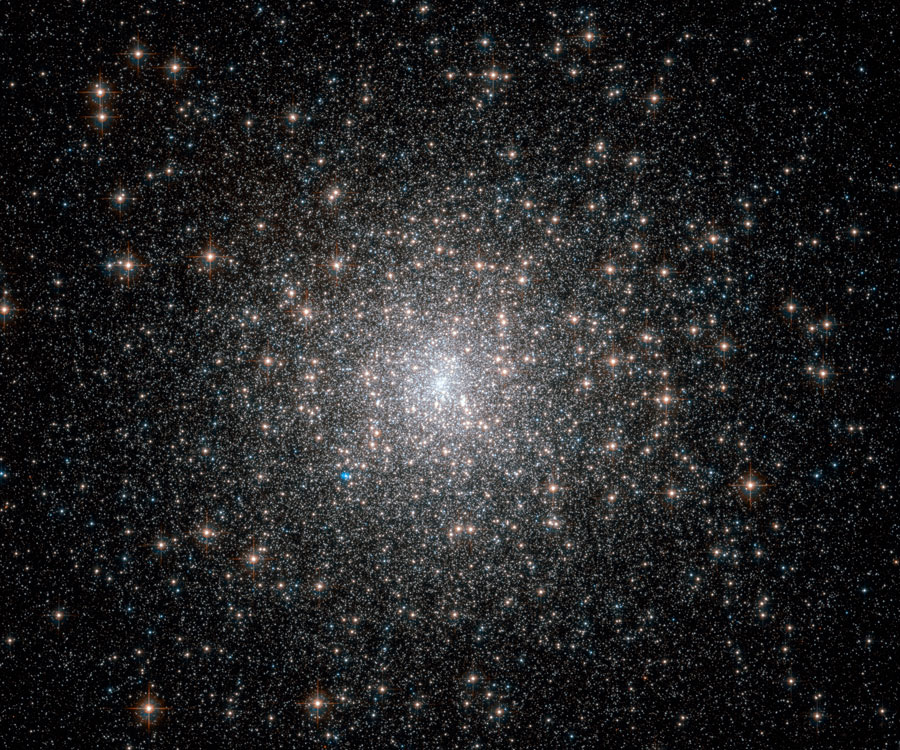
\includegraphics[width=12cm]{images/m15.jpg}
\caption[M]{G}
\end{figure}

T 

\begin{equation}
I(R)\sigma_{p}^{2}(R)=\frac{2}{\Gamma}\int_{R}^{\infty}\left(1-\beta\frac{R^{2}}{r^{2}}\right)\frac{\nu\bar{v_{r}^{2}}rdr}{\sqrt{r^{2}-R^{2}}}
\end{equation}

Whuster.  

\section{Gravitational Lensing}

At small radii, stars dominate the lensing mass, so that lensing provides a direct probe of the stellar mas to light ratio, with only small corrections needed for darl matter.

In the paper of Russell Smith (a giant elliptical galaxy with a lightweight initial mass funciton) they find a stellar mass to light ratio of 3.01 plus minus 0.25

Modelling the lensing configuration provides the total projection mass within an aperture.

bulges have heavier IMFs than disks

Several recent studies have presented evidence for "heavyweight" IMFs in giant ellipticals, with a mass-to-light-ratio twice that of a Milky Way like IMF.



\section{IMF in BCGs}



